\documentclass[12pt,fleqn,a4paper]{report}
%\documentclass[12pt,fleqn,a4paper,draft]{report}
\usepackage[brazil]{babel}
\usepackage[utf8]{inputenc} 
%------------------------------------------------------
\usepackage{caption}
\usepackage{algorithm}
\usepackage{algpseudocode}
%\usepackage[compact]{titlesec}
\usepackage{indentfirst}
%------------------------------------------------------

\usepackage{graphicx}
\usepackage{amssymb}
\usepackage{amsmath,amsfonts,amscd,bezier,amstext}
\usepackage{colortbl}
\usepackage{setspace}
\usepackage{pxfonts}
\usepackage{subfigure,float,subfloat}
\usepackage{textcomp}
\usepackage{boxedminipage}
\usepackage{algorithm}
\usepackage[brazil,pagebackref,colorlinks,linkcolor=black,citecolor=black]{hyperref}
\usepackage{multirow}
\usepackage{booktabs}
\usepackage{textcomp}
\usepackage{enumitem}
\usepackage{mathtools}
\usepackage[title]{appendix}
\usepackage{animate}
\usepackage{rotating} %% permite rotacionar objetos do tipo ``floating''
%\usepackage{subfig}
\usepackage[flushleft]{threeparttable}
\usepackage{xcolor}
\usepackage{microtype}
\usepackage{icomma}
\usepackage{fancyvrb}
\usepackage{fancyhdr}
\usepackage{longtable}
\usepackage{caption}
\usepackage{stackengine}
\usepackage{nomencl}
\usepackage{ifthen}
\usepackage{makecell}
\usepackage{scalerel}
\usepackage{here}
\usepackage{marvosym}			% Alguns símbolos
\usepackage{wasysym}			% Alguns símbolos
\usepackage[alf,abnt-etal-list=0,abnt-etal-text=it,abnt-emphasize=it,bibjustif,abnt-last-names=bibtex,abnt-url-package=url]{abntex2cite}
\usepackage{filecontents}
\usepackage{lscape}
\usepackage{color}
\usepackage{pgf}
\usepackage{tikz}
\usepackage{ragged2e}
%\usepackage{cleveref}
%\usepackage[brazilian,hyperpageref]{backref}	 % Paginas com as citações na bibl

% ---
% Configurações do pacote backref
% Usado sem a opção hyperpageref de backref
\renewcommand{\backrefpagesname}{Citado na(s) página(s):~}
% Texto padrão antes do número das páginas
\renewcommand{\backref}{}
% Define os textos da citação
\renewcommand*{\backrefalt}[4]{
	\ifcase #1 %
		Nenhuma citação no texto.%
	\or
		Citado na página #2.%
	\else
		Citado #1 vezes, nas páginas #2.%
	\fi}%
% ---

\usetikzlibrary{shapes,arrows}
%
%\pdfminorversion=5 
%\pdfcompresslevel=9
%\pdfobjcompresslevel=9
%\setlength{\textheight}{24cm} \setlength{\textwidth}{16cm}
%\voffset=-1.5cm \hoffset=-1.2cm
\DeclareGraphicsExtensions{.JPG,.jpg,.tiff,.pdf,.mps,.PNG,.png}

%\newfloat{algorithm}{!ht}{loa}
%\floatname{algorithm}{Algorithm}

\DeclareMathOperator{\sen}{sen}
\usepackage[normalem]{ulem}

\usepackage{color}
\definecolor{dkgreen}{rgb}{0,0.6,0}
\definecolor{gray}{rgb}{0.5,0.5,0.5}
\definecolor{mauve}{rgb}{0.58,0,0.82}
\newcommand{\mltc}[3]{\multicolumn{#1}{#2}{#3}}
\newcommand{\mltr}[2]{\multirow{#1}{*}{#2}}
\newcommand{\done}[2]{\frac{\partial{#1}}{\partial{#2}}}
\newcommand{\dtwo}[2]{\frac{\partial{^2#1}}{\partial{#2}^2}}
\newcommand{\dtwotwo}[3]{\frac{\partial{^2#1}}{\partial{#2}\partial{#3}}}
\newcommand{\dn}[3]{\frac{\partial{^{#3}#1}}{\partial{#2}^{#3}}}

%=============================================================
%============== Formatação dos códigos =======================
%=============================================================
% ---> Inserir códigos
\usepackage{listings}		
% ---> Aceitar acentos nos códigos
\usepackage{listingsutf8}		 
\lstset{inputencoding=utf8/latin1}

% ---> Definição dos acentos para o listings:
\lstset{
	literate=%
	{é}{{\'{e}}}1
	{è}{{\`{e}}}1
	{ê}{{\^{e}}}1
	{ë}{{\¨{e}}}1
	{É}{{\'{E}}}1
	{Ê}{{\^{E}}}1
	{û}{{\^{u}}}1
	{ù}{{\`{u}}}1
	{ú}{{\'{u}}}1
	{â}{{\^{a}}}1
	{à}{{\`{a}}}1
	{á}{{\'{a}}}1
	{ã}{{\~{a}}}1
	{Á}{{\'{A}}}1
	{Â}{{\^{A}}}1
	{Ã}{{\~{A}}}1
	{ç}{{\c{c}}}1
	{Ç}{{\c{C}}}1
	{õ}{{\~{o}}}1
	{ó}{{\'{o}}}1
	{ô}{{\^{o}}}1
	{Õ}{{\~{O}}}1
	{Ó}{{\'{O}}}1
	{Ô}{{\^{O}}}1
	{î}{{\^{i}}}1
	{Î}{{\^{I}}}1
	{í}{{\'{i}}}1
	{Í}{{\~{Í}}}1
}

\lstset{language=[90]Fortran,
	basicstyle=\tiny,
	numbers=left,
	frame=shadowbox,
	showstringspaces=false,
	rulesepcolor=\color{black}}

\renewcommand{\lstlistingname}{Código}

%=============================================================
%=============================================================

\pagestyle{fancy}
\fancyhf{}
\usepackage[top=2.0 cm,left=2 cm,right=2 cm,bottom=2.0 cm,includeheadfoot,headheight=30pt]{geometry} %Formata as margens do textos
\rhead{
\includegraphics[width=1cm]{layout_document/ufu.pdf}}
\lhead{Relatório Técnico Parcial 2}
\rfoot{ \thepage}
% Redefine the plain page style
\fancypagestyle{plain}{
	\fancyhf{}
	\rfoot{ \thepage}
	\rhead{
\includegraphics[width=1cm]{layout_document/ufu.pdf}}
	\lhead{Relatório Técnico Parcial 2}
}
\fancypagestyle{capa}{
	\fancyhf{}
}

% Length to control the \fancyheadoffset and the calculation of \headline
% simultaneously
\newlength\FHoffset
\setlength\FHoffset{0cm}

\addtolength\headwidth{2\FHoffset}

\fancyheadoffset{\FHoffset}

% these lengths will control the headrule trimming to the left and right 
\newlength\FHleft
\newlength\FHright

% here the trimmings are controlled by the user
\setlength\FHleft{0cm}
\setlength\FHright{0cm}

%\pagestyle{fancy}
%\fancyhf{}
%%\usepackage[top=2.0 cm,left=3.5 cm,right=3.0 cm,bottom=2.0 cm,includeheadfoot]{geometry} %Formata as margens do textos
%\usepackage[top=2.0 cm,left=2 cm,right=2 cm,bottom=2.0 cm,includeheadfoot,headheight=30pt]{geometry} %Formata as margens do textos
%\rhead{
\includegraphics[width=1cm]{layout_document/ufu.pdf}}
%\lhead{Relatório técnico parcial}
%\rfoot{ \thepage}
%% Redefine the plain page style
%\fancypagestyle{plain}{
%	\fancyhf{}
%	\rfoot{ \thepage}
%	\rhead{
\includegraphics[width=1cm]{layout_document/ufu.pdf}}
%	\lhead{Relatório técnico parcial}
%}
%\fancypagestyle{capa}{
%	\fancyhf{}
%}

\addto\captionsportugues{% Replace "english" with the language you use
	\renewcommand{\contentsname}%
	{Sumário}%
}

\newcommand{\figuraabnt}[6]{
	\begin{figure}[H]
		\centering
		\caption{#1}
		\centering
		\begin{tabular}{c}
			{\includegraphics[trim={#2},clip,width=#3\linewidth]{#4}}\\
			\multicolumn{1}{l}{\footnotesize{Fonte: #5}}\\
		\end{tabular}
		\label{#6}
	\end{figure}
}

\newcommand{\duasfigurasabnt}[9]{
	\begin{figure}[H]
		\centering
		\caption{#1}
		\centering
		\begin{tabular}{c c}
			{\includegraphics[width= #3 \linewidth]{#4}} & {\includegraphics[width= #6 \linewidth]{#7}}\\
			{#2}&{#5}\\
			\multicolumn{2}{l}{\footnotesize{Fonte: #8}} \\
		\end{tabular}
%	    \legend{Fonte: #8}
		\label{#9}
	\end{figure}
	
}


\usepackage{float}
\usepackage{caption}

\newfloat{grafico}{htpb}{grf}[figure]
\floatstyle{plaintop}
\restylefloat{grafico}
\renewcommand\thegrafico{\arabic{grafico}}
\newcommand{\graficoname}{Gr\'{a}fico}
\floatname{grafico}{\graficoname}

\newcommand{\listofgraficoname}{Lista de gráficos}
\newcommand{\listofgrafico}{%
%	\addcontentsline{toc}{chapter}{\listofgraficoname}
	\listof{grafico}{\listofgraficoname}
}
\newcounter{graficocount}

\newcommand{\doisgraficosabnt}[9]{
	
	 \setcounter{grafico}{\value{graficocount}}
	 
	\begin{grafico}[H]

		\caption[Gráfico \ref{#9}~--~#1]{#1\label{#9}}
		\centering
		\begin{tabular}{c c}
			{\includegraphics[width= #3 \linewidth]{#4}} & {\includegraphics[width= #6 \linewidth]{#7}}\\
			{\footnotesize{#2}}&{\footnotesize{#5}}\\
			\multicolumn{2}{l}{\footnotesize{Fonte: #8}}
		\end{tabular}
		
	\end{grafico}
	\stepcounter{graficocount}
}


\newcommand{\doisgraficosabntcoluna}[9]{
	
	\setcounter{grafico}{\value{graficocount}}
	
	\begin{grafico}[H]
		
		\caption[Gráfico \ref{#9}~--~#1]{#1\label{#9}}
		\centering
		\begin{tabular}{c}
			{\includegraphics[width= #3 \linewidth]{#4}}\\
			{\footnotesize{#2}}\\
			{\includegraphics[width= #6 \linewidth]{#7}}\\
			{\footnotesize{#5}}\\
			\multicolumn{1}{l}{\footnotesize{Fonte: #8}}
		\end{tabular}
		
	\end{grafico}
	\stepcounter{graficocount}
}



\newcommand{\graficoabnt}[5]{
	 \setcounter{grafico}{\value{graficocount}}
	\begin{grafico}[H]
		
		\caption[Gráfico \ref{#5}~--~#1]{#1\label{#5}}
		\centering
		\begin{tabular}{c c}
			\multicolumn{2}{c}{\includegraphics[width= #2 \linewidth]{#3}}\\
			\multicolumn{2}{l}{\footnotesize{Fonte: #4}}
		\end{tabular}
		
	\end{grafico}
	\stepcounter{graficocount}
}
\newcommand{\nasa}{elaborada pelo autor.}
\newcommand{\nasas}{elaboradas pelo autor.}
\newcommand{\naso}{elaborado pelo autor.}
\newcommand{\nasos}{elaborados pelo autor.}

\newcommand{\nasavisit}{\nasa{} Captura de tela do software VisIt \cite{visit}.}
\newcommand{\nasasvisit}{\nasas{} Capturas de tela do software VisIt \cite{visit}.}
\newcommand{\nasaanflex}{\nasa{} Captura de tela do software Anflex \cite{anflex}.}

\newcommand{\nasapara}{\nasa{} Captura de tela do software Paraview \cite{paraview}.}
\newcommand{\nasaspara}{\nasas{} Capturas de tela do software Paraview \cite{paraview}.}

\newcommand{\nasomatplot}{\naso{} Gráfico gerado com Matplotlib \cite{matplotlib}.}
\newcommand{\nasosmatplot}{\nasos{} Gráficos gerados com Matplotlib \cite{matplotlib}.}

\newcommand{\nasamatplot}{\nasa{} Figura gerada com Matplotlib \cite{matplotlib}.}
\newcommand{\nasasmatplot}{\nasas{} Figuras geradas com Matplotlib \cite{matplotlib}.}

\newcommand{\Fonte}[2]{\multicolumn{#1}{l}{\footnotesize{Fonte: #2}}}
\newcommand{\Fontefig}[1]{\flushleft\footnotesize{Fonte: #1}}
\newcommand{\adaptado}[1]{adaptado de \citeonline{#1}.}
\newcommand{\adaptada}[1]{adaptada de \citeonline{#1}.}

%%%%%%%%%%%%%%%%FIGURAS%%%%%%%%%%%%%%

%Ao longo do texto

\newcommand{\fig}[1]{\hyperref[{#1}]{Fig. \ref{#1}}}
\newcommand{\figs}[2]{Figs. \ref{#1} e \ref{#2}}
\newcommand{\figstres}[3]{Figs. \ref{#1}, \ref{#2} e \ref{#3}}
\newcommand{\figsquatro}[4]{Figs. \ref{#1}, \ref{#2}, \ref{#3} e \ref{#4}}

%Início de frase:

\newcommand{\figini}[1]{\hyperref[{#1}]{Figura \ref{#1}}}
\newcommand{\figsini}[2]{Figuras \ref{#1} e \ref{#2}}
\newcommand{\figsiniquatro}[4]{Figuras \ref{#1}, \ref{#2}, \ref{#3} e \ref{#4}}

%%%%%%%%%%%%%%%%GRAFICOS%%%%%%%%%%%%%%

%Ao longo do texto

\newcommand{\graf}[1]{\hyperref[{#1}]{Gráf. \ref{#1}}}
\newcommand{\grafs}[2]{Gráfs. \ref{#1} e \ref{#2}}

%Início de frase:

\newcommand{\grafini}[1]{\hyperref[{#1}]{Gráfico \ref{#1}}}
\newcommand{\grafsini}[2]{Gráficos \ref{#1} e \ref{#2}}


%%%%%%%%%%%%%%%%TABELAS%%%%%%%%%%%%%%

%Ao longo do texto

\newcommand{\tab}[1]{\hyperref[{#1}]{Tab. \ref{#1}}}
\newcommand{\tabs}[2]{Tabs. \ref{#1} e \ref{#2}}

%Início de frase:

\newcommand{\tabini}[1]{\hyperref[{#1}]{Tabela \ref{#1}}}
\newcommand{\tabsini}[2]{Tabelas \ref{#1} e \ref{#2}}

%%%%%%%%%%%%%%%%EQUAÇÕES%%%%%%%%%%%%%%

%Ao longo do texto

\newcommand{\eq}[1]{\hyperref[{#1}]{Eq. (\ref{#1})}}
\newcommand{\eqsa}[2]{Eqs. (\ref{#1}) a (\ref{#2})}
\newcommand{\eqs}[2]{Eqs. (\ref{#1}) e (\ref{#2})}
\newcommand{\eqsquatro}[4]{Eqs. (\ref{#1}), (\ref{#2}), (\ref{#3}) e (\ref{#4})}
\newcommand{\eqsoito}[8]{Eqs. (\ref{#1}), (\ref{#2}), (\ref{#3}), (\ref{#4}), (\ref{#5}), (\ref{#6}), (\ref{#7}), (\ref{#8})}

%Início de frase:

\newcommand{\eqini}[1]{\hyperref[{#1}]{Equação (\ref{#1})}}
\newcommand{\eqsini}[2]{Equações (\ref{#1}) e (\ref{#2})}

%%%%%%%%%%%%%%%%ANEXO%%%%%%%%%%%%%%

%\newcommand{\refanexo}[1]{ANEXO \ref{#1}}

\newcommand*{\refanexo}[1]{\hyperref[{#1}]{ANEXO~\ref*{#1}}}
%%%%%%%%%%%%%%%%APÊNDICE%%%%%%%%%%%%%%

%\newcommand{\refapendice}[1]{AP\^{E}NDICE \ref{#1}}

\newcommand*{\refapendice}[1]{\hyperref[{#1}]{AP\^{E}NDICE~\ref*{#1}}}

%%%%%%%%%%%%%%%%Seção%%%%%%%%%%%%%%

\newcommand*{\refsec}[1]{\hyperref[{#1}]{seção~\ref*{#1}}}
\newcolumntype{C}[1]{>{\centering\let\newline\\\arraybackslash\hspace{0pt}}m{#1}}

\newcommand{\stkout}[1]{\ifmmode\text{\sout{\ensuremath{#1}}}\else\sout{#1}\fi} % cortar uma letra

\newcommand{\reg}[1]{#1$^{\tiny{\circledR}}$} % Símbolo de marca registrada

\newcommand{\MFSim}{MFSim}

\newcommand{\PETSc}{\textit{PETSc}}
%\usepackage{subcaption}
\usepackage{pgfplots}
\usetikzlibrary{spy,calc}


\newif\ifblackandwhitecycle
\gdef\patternnumber{0}

\pgfkeys{/tikz/.cd,
    zoombox paths/.style={
        draw=orange,
        very thick
    },
    black and white/.is choice,
    black and white/.default=static,
    black and white/static/.style={ 
        draw=white,   
        zoombox paths/.append style={
            draw=white,
            postaction={
                draw=black,
                loosely dashed
            }
        }
    },
    black and white/static/.code={
        \gdef\patternnumber{1}
    },
    black and white/cycle/.code={
        \blackandwhitecycletrue
        \gdef\patternnumber{1}
    },
    black and white pattern/.is choice,
    black and white pattern/0/.style={},
    black and white pattern/1/.style={    
            draw=white,
            postaction={
                draw=black,
                dash pattern=on 2pt off 2pt
            }
    },
    black and white pattern/2/.style={    
            draw=white,
            postaction={
                draw=black,
                dash pattern=on 4pt off 4pt
            }
    },
    black and white pattern/3/.style={    
            draw=white,
            postaction={
                draw=black,
                dash pattern=on 4pt off 4pt on 1pt off 4pt
            }
    },
    black and white pattern/4/.style={    
            draw=white,
            postaction={
                draw=black,
                dash pattern=on 4pt off 2pt on 2 pt off 2pt on 2 pt off 2pt
            }
    },
    zoomboxarray inner gap/.initial=5pt,
    zoomboxarray columns/.initial=2,
    zoomboxarray rows/.initial=2,
    subfigurename/.initial={},
    figurename/.initial={zoombox},
    zoomboxarray/.style={
        execute at begin picture={
            \begin{scope}[
                spy using outlines={%
                    zoombox paths,
                    width=\imagewidth / \pgfkeysvalueof{/tikz/zoomboxarray columns} - (\pgfkeysvalueof{/tikz/zoomboxarray columns} - 1) / \pgfkeysvalueof{/tikz/zoomboxarray columns} * \pgfkeysvalueof{/tikz/zoomboxarray inner gap} -\pgflinewidth,
                    height=\imageheight / \pgfkeysvalueof{/tikz/zoomboxarray rows} - (\pgfkeysvalueof{/tikz/zoomboxarray rows} - 1) / \pgfkeysvalueof{/tikz/zoomboxarray rows} * \pgfkeysvalueof{/tikz/zoomboxarray inner gap}-\pgflinewidth,
                    magnification=3,
                    every spy on node/.style={
                        zoombox paths
                    },
                    every spy in node/.style={
                        zoombox paths
                    }
                }
            ]
        },
        execute at end picture={
            \end{scope}
%            \node at (image.north) [anchor=north,inner sep=0pt] {\subcaptionbox{\label{\pgfkeysvalueof{/tikz/figurename}-image}}{\phantomimage}};
%            \node at (zoomboxes container.north) [anchor=north,inner sep=0pt] {\subcaptionbox{\label{\pgfkeysvalueof{/tikz/figurename}-zoom}}{\phantomimage}};
     \gdef\patternnumber{0}
        },
        spymargin/.initial=0.5em,
        zoomboxes xshift/.initial=1,
        zoomboxes right/.code=\pgfkeys{/tikz/zoomboxes xshift=1},
        zoomboxes left/.code=\pgfkeys{/tikz/zoomboxes xshift=-1},
        zoomboxes yshift/.initial=-0.3,
        zoomboxes above/.code={
            \pgfkeys{/tikz/zoomboxes yshift=1},
            \pgfkeys{/tikz/zoomboxes xshift=0}
        },
        zoomboxes below/.code={
            \pgfkeys{/tikz/zoomboxes yshift=-1},
            \pgfkeys{/tikz/zoomboxes xshift=0}
        },
        caption margin/.initial=4ex,
    },
    adjust caption spacing/.code={},
    image container/.style={
        inner sep=0pt,
        at=(image.north),
        anchor=north,
        adjust caption spacing
    },
    zoomboxes container/.style={
        inner sep=0pt,
        at=(image.north),
        anchor=north,
        name=zoomboxes container,
        xshift=\pgfkeysvalueof{/tikz/zoomboxes xshift}*(\imagewidth+\pgfkeysvalueof{/tikz/spymargin}),
        yshift=\pgfkeysvalueof{/tikz/zoomboxes yshift}*(\imageheight+\pgfkeysvalueof{/tikz/spymargin}+\pgfkeysvalueof{/tikz/caption margin}),
        adjust caption spacing
    },
    calculate dimensions/.code={
        \pgfpointdiff{\pgfpointanchor{image}{south west} }{\pgfpointanchor{image}{north east} }
        \pgfgetlastxy{\imagewidth}{\imageheight}
        \global\let\imagewidth=\imagewidth
        \global\let\imageheight=\imageheight
        \gdef\columncount{1}
        \gdef\rowcount{1}
        \gdef\zoomboxcount{1}
    },
    image node/.style={
        inner sep=0pt,
        name=image,
        anchor=south west,
        append after command={
            [calculate dimensions]
            node [image container,subfigurename=\pgfkeysvalueof{/tikz/figurename}-image] {\phantomimage}
            node [zoomboxes container,subfigurename=\pgfkeysvalueof{/tikz/figurename}-zoom] {\phantomimage}
        }
    },
    color code/.style={
        zoombox paths/.append style={draw=#1}
    },
    connect zoomboxes/.style={
    spy connection path={\draw[draw=none,zoombox paths] (tikzspyonnode) -- (tikzspyinnode);}
    },
    help grid code/.code={
        \begin{scope}[
                x={(image.south east)},
                y={(image.north west)},
                font=\footnotesize,
                help lines,
                overlay
            ]
            \foreach \x in {0,1,...,9} { 
                \draw(\x/10,0) -- (\x/10,1);
                \node [anchor=north] at (\x/10,0) {0.\x};
            }
            \foreach \y in {0,1,...,9} {
                \draw(0,\y/10) -- (1,\y/10);                        \node [anchor=east] at (0,\y/10) {0.\y};
            }
        \end{scope}    
    },
    help grid/.style={
        append after command={
            [help grid code]
        }
    },
}

\newcommand\phantomimage{%
    \phantom{%
        \rule{\imagewidth}{\imageheight}%
    }%
}
\newcommand\zoombox[2][]{
    \begin{scope}[zoombox paths]
        \pgfmathsetmacro\xpos{
            (\columncount-1)*(\imagewidth / \pgfkeysvalueof{/tikz/zoomboxarray columns} + \pgfkeysvalueof{/tikz/zoomboxarray inner gap} / \pgfkeysvalueof{/tikz/zoomboxarray columns} ) + \pgflinewidth
        }
        \pgfmathsetmacro\ypos{
            (\rowcount-1)*( \imageheight / \pgfkeysvalueof{/tikz/zoomboxarray rows} + \pgfkeysvalueof{/tikz/zoomboxarray inner gap} / \pgfkeysvalueof{/tikz/zoomboxarray rows} ) + 0.5*\pgflinewidth
        }
        \edef\dospy{\noexpand\spy [
            #1,
            zoombox paths/.append style={
                black and white pattern=\patternnumber
            },
            every spy on node/.append style={#1},
            x=\imagewidth,
            y=\imageheight
        ] on (#2) in node [anchor=north west] at ($(zoomboxes container.north west)+(\xpos pt,-\ypos pt)$);}
        \dospy
        \pgfmathtruncatemacro\pgfmathresult{ifthenelse(\columncount==\pgfkeysvalueof{/tikz/zoomboxarray columns},\rowcount+1,\rowcount)}
        \global\let\rowcount=\pgfmathresult
        \pgfmathtruncatemacro\pgfmathresult{ifthenelse(\columncount==\pgfkeysvalueof{/tikz/zoomboxarray columns},1,\columncount+1)}
        \global\let\columncount=\pgfmathresult
        \ifblackandwhitecycle
            \pgfmathtruncatemacro{\newpatternnumber}{\patternnumber+1}
            \global\edef\patternnumber{\newpatternnumber}
        \fi
    \end{scope}
}

%EX:

%		\begin{figure}[ht]
%			\centering
%			\caption{Geometria gerada para o \textit{riser} analisado (modelo 5).}
%			\begin{tikzpicture}[
%				zoomboxarray,
%			    zoomboxes right,
%			    zoomboxarray columns=2,
%			    zoomboxarray rows=3,
%			    connect zoomboxes,
%			    zoombox paths/.append style={ultra thick, black}]
%			    \node [image node] { \includegraphics[width=0.45\textwidth]{marcelo/figures/SegmentedStrake}};
%			    \zoombox[magnification=2]{0.5,0.7}
%			\end{tikzpicture}
%		\end{figure}
%		
%		\begin{figure}[h]
%		\centering
%		\caption{Geometria gerada para o \textit{riser} analisado (modelo 5).}
%			\begin{tikzpicture}[zoomboxarray,black and white=cycle,connect zoomboxes]
%			    \node [image node] { \includegraphics[width=0.45\textwidth]{marcelo/figures/SegmentedStrake} };
%			    \zoombox[magnification=2]{0.5,0.8}
%	%		    \zoombox[color code=red,magnification=6]{0.4,0.83}
%	%		    \zoombox{0.42,0.45}
%	%		    \zoombox[magnification=5]{0.95,0.52}
%			\end{tikzpicture}
%		\end{figure}
%		
%		\newpage

\begin{document}

	\baselineskip 25pt
	\thispagestyle{empty}
	
	\begin{singlespace}
	
		\begin{figure}[htb]
			\begin{center}
				
\includegraphics[scale=0.7]{layout_document/ufu.pdf}\\
				{\bf Universidade Federal de Uberl\^andia}
			\end{center}
		\end{figure}
		
		\begin{figure}[htb]
			\begin{minipage}{0.49\linewidth}
				\centering
				
\includegraphics[scale=0.15]{layout_document/lmest.pdf}\\
				{\bf \small{Laborat\'orio de Mec\^anica de Estruturas}} \\
				{\bf \small{Jos\'e Eduardo Tann\'us Reis}}
			\end{minipage}
			\begin{minipage}{0.49\linewidth}
				\centering
				\vspace{-0.15cm}
\includegraphics[scale=0.22]{layout_document/mflab.pdf}\\ \vspace{0.15cm}
				{\bf \small{Laborat\'orio de Mec\^anica dos Fluidos}}
			\end{minipage}
		\end{figure}
	
	\end{singlespace}
	%\vspace*{30 pt}
	
	\begin{large}
		\begin{center}
			Relatório Técnico Parcial 2\\
			\vspace*{10 pt}
			Período: 01/01/2020 à 31/08/2020\\
			\vspace*{25 pt}
			{\bf Desenvolvimento de uma ferramenta computacional dedicada à construção de metamodelos de estruturas submersas}
		\end{center}
	\end{large}
	
	\vspace*{10 pt}
	\begin{normalsize}
		\begin{description}
			\item[] 
	
			\hspace{0.7cm} UNIVERSIDADE FEDERAL DE UBERLÂNDIA - UFU\\
			FUNDA\c C\~AO DE APOIO UNIVERSITÁRIO - FAU
			\begin{flushleft}
				Termo de Cooperação: PT-127.01.13870 \\
				Número SAP: 4600585313 \\
				Número SIC: 2019/00056-2 \\
				Número jurídico: 5900.0111467.19.9\\
				Data de Assinatura: 31 de maio de 2019\\
				Data de Término Prevista: 29 de maio de 2021
			\end{flushleft}
	
			\vspace{10pt}
			\item[Coordenador:] Prof. Dr. Aldemir Aparecido Cavalini Jr  
			\vspace{10pt}
			\item[Gerencia Técnica:] CENPES/PDDP/TDUT
			\item[Interlocutor Técnico:] Marcos André Duarte Martins
	
		\end{description}
	\end{normalsize}
	
	\newpage
	
	\section*{Equipe Responsável}

		\begin{normalsize}
			\begin{description}
				\vspace{20pt}
				\item[Coordenador:] Prof. Dr. Aldemir Aparecido Cavalini Jr 
				\item[\vspace{10pt}]  
		
				\item[Pesquisadores:] Prof. Dr. Aristeu da Silveira Neto \\
				\hspace*{1.95cm} Prof. Dr. João Marcelo Vedovoto \\
				\hspace*{1.95cm} Dra. Denise Kinoshita \\
				\hspace*{1.95cm} Dr. Marcelo Maia Ribeiro Damasceno \\
				\hspace*{1.95cm} Msc. Hélio Ribeiro Neto \\
				\hspace*{1.95cm} Msc. Tatiane Nunes da Costa \\
				\hspace*{1.95cm} Eng. André Rezende Dessimoni Carvalho \\
				\hspace*{1.95cm} Eng. Bruno Resende Ferreira Rende\\
				\hspace*{1.95cm} Alessandra Lopes Paiva\\
				\hspace*{1.95cm} Arturo Burgos Moreira\\
				\hspace*{1.95cm} Felipe José Oliveira Ribeiro\\
		
				\item[Responsável da Convenente:] Gisele Debortoli Guilherme
				 
				\item[Gerencia Técnica:] CENPES/PDDP/TDUT
				\item[Interlocutor Técnico:] Marcos André Duarte Martins
			\end{description}
		\end{normalsize}

		\newpage
	\section*{Resumo}
	
		\noindent O presente relatório técnico parcial corresponde às atividades realizadas durante o período de janeiro de 2020 -- agosto de 2020, a respeito do projeto \textit{Desenvolvimento de uma Ferramenta Computacional Dedicada à Construção de Metamodelos de Estruturas Submersas} sob o termo de cooperação PT-127.01.13870 / SAP 4600585313. Devido ao caráter multidisciplinar do presente projeto de pesquisa, este relatório é dividido em capítulos (quase) independentes, cada qual com sua metodologia, discussões e resultados específicos. Como regra geral, os desenvolvimentos seguiram as linhas: \textcolor{red}{\textbf{CONCLUIR CONCLUIR CONCLUIR CONCLUIR CONCLUIR CONCLUIR CONCLUIR}}.
	
	\newpage
	\tableofcontents
	\newpage
	
	%\include{informacoes}
	%\include{objetivos}
	
	%\setcounter{page}{2}
	%\tableofcontents \pagestyle{plain}
	
	\chapter{Introdução}

\noindent 

	A simulação computacional é uma ferramenta de emprego crescente, que não se limita ao domínio da engenharia, sendo ampliada para aplicações em diversos setores da ciência contemporânea. Já é possível modelar simulações para campos aerodinâmicos, biológicos, meteorológicos e até financeiros. Tal recurso é extremamente útil para a compreensão de fenômenos complexos, de variadas amplitudes no domínio temporal e para a economia de recursos e tempo em projetos de engenharia.
	
	A engenharia moderna possui como alguns dos principais desafios a otimização de sistemas já existentes e a modelagem de novos sistemas com excelentes rendimentos mecânico e térmico. Ainda, essas melhorias devem ocorrer em paralelo com um baixo custo associado de forma a manter a competitividade no mercado. Antes do avanço tecnológico das últimas décadas, a resolução de problemas físicos demandava um grande esforço e custo em função da necessidade de reprodução material, mas esse método pôde ser substituido com teorias bem trabalhadas e fundamentadas em experimentações passadas, modelagens físicas e matemáticas aplicadas em uma resolução numérica-computacional.
	
	Dentre os vários ramos da engenharia, a mecânica dos fluidos é um grande exemplo de aplicação dos métodos supracitados. Tópicos como turbulência, troca de calor e interação fluido-estrutura são trabalhados de forma extensiva na pesquisa, e têm apresentado resultados muito coerentes com aqueles observados pelo método empírico. 
	
	Este trabalho objetiva a execução de análises matemáticas e discretizações numéricas para os transportes por difusão e advecção para os casos unidimensional e bidimensional, sob a metodologia explícita e implícita. Tais mecanismos são observados na transferência de energia térmica em escoamentos laminares, de transição e turbulentos em proporções particulares para cada caso. Os diferentes tratamentos do termo temporal são trabalhados de forma conjunta para a comparação da relação entre custo computacional e estabilidade numérica de ambos. A partir da modelagem numérica das equações associadas, se produz um código, ou modelo computacional, que resolve numericamente o problema a partir de uma condição inicial e condições de contorno conhecidas, finalmente comparando a solução numérica com a analítica.
	
	%Por fim, escoamentos heterogêneos, também tratados neste trabalho, são de grande importância para a mecânica dos fluidos devido à sua extensa ocorrência na prática da engenharia mecânica. O estudo de tais escoamentos possibilita uma modelagem de carregamento de particulado com o fluido durante a extração de petróleo ou a troca de calor em um líquido em transição de fase, por exemplo.
	
\newpage
	

 \section{Metodologia}
 % --------------------------------------------------------------------------

\noindent

	A metodologia proposta para o presente trabalho de iniciação científica se baseia
na definição de problemas, estudando primeiramente os casos particulares, e uma vez
compreendida a natureza do conteúdo, seguindo para problemas mais gerais e complexos.

	Inicialmente verifica-se na literatura as dinâmicas envolvidas nos mecanismos propostos para este estudo. A partir das relações obtidas nessa revisão, elabora-se uma discretização a partir de métodos numéricos e realiza-se a implementação dos mesmos em um código computacional. As rotinas são confeccionadas na linguagem de programação Fortran, para familiarização do aluno com a linguagem base dos códigos do Laboratório de Mecânica dos Fluidos Computacional (MFLab) da Faculdade de Engenharia Mecânica (FEMEC) da Universidade Federal de Uberlândia.
 

\subsection{Difusão}

\noindent

	A difusão é um mecanismo de transporte que possui diferentes definições nos campos da química, biologia e física. Especificamente para o caso de transferência de calor, a difusão é bem definida matematicamente por uma equação diferencial parcial (EDP), que envolve uma derivada parcial de primeira ordem no domínio temporal e uma derivada parcial de segunda ordem no domínio espacial. Os termos são relacionados, através de uma constante (difusividade), à um termo fonte, resultante da diferença desses elementos, como indicado na Eq. (\ref{Difusaoone}).
	
\begin{align}
 \label{Difusaoone}
 f(x,y,z,t) = \dfrac{\partial \phi}{\partial t} - \alpha \nabla^2 \phi
\end{align}

	Assim, para o caso unidimensional, obtém-se a relação dada pela Eq.(\ref{Difuni}).
	
\begin{align}
 \label{Difuni}
 f(x,t) = \dfrac{\partial \phi}{\partial t} - \alpha \left(\dfrac{\partial^2 \phi}{\partial x^2}\right)
\end{align}

	E para o caso bidimensional, obtém-se a relação dada pela Eq.(\ref{Difbi}).
	
\begin{align}
 \label{Difbi}
 f(x,y,t) = \dfrac{\partial \phi}{\partial t} - \alpha \left[ \left(\dfrac{\partial^2 \phi}{\partial x^2}\right) - \left(\dfrac{\partial^2 \phi}{\partial y^2}\right)\right]
\end{align}
	
	A difusividade ($\alpha$) é traduzida fisicamente como a rapidez com que a energia térmica é transportada espacialmente para dado material. O termo fonte ($f$), por sua vez, se traduz na resultante da diferença das parciais, que deve ser nulo para a solução da difusão. 

\subsection{Advecção}

\noindent

	A advecção é um mecanismo de transporte que também é presente em vários campos de estudo, dado pela transferência de calor juntamente com a transferência de espécie. Esse fenômeno é modelado matemáticamente pela Eq. (\ref{Adveccao}).
	
\begin{align}
\label{Adveccao}
f(x,y,z,t) = \dfrac{\partial \phi}{\partial t} + c \nabla \phi
\end{align}

	Para o caso unidimensional, de forma análoga ao caso da difusão, tem-se que a relação fica como indicada pela Eq. (\ref{advuni}).
	
\begin{align}
\label{advuni}
f(x,t) = \dfrac{\partial \phi}{\partial t} + c \dfrac{\partial \phi}{\partial x}
\end{align}

	Para o caso bidimensional, obtém-se a relação dada pela Eq. (\ref{advbi}).
	
\begin{align}
\label{advbi}
f(x,t) = \dfrac{\partial \phi}{\partial t} + cx \dfrac{\partial \phi}{\partial x} + cy \dfrac{\partial \phi}{\partial y}
\end{align}
	
	A velocidade ($c$) é traduzida fisicamente como a velocidade com que a variação térmica ocorre com a movimentação de massa na direção avaliada, sendo que essa velocidade pode ser positiva ou negativa. Já o termo fonte ($f$), se traduz na resultante da soma das parciais, que deve ser nulo para a solução da difusão.

\subsection{Difusão e Advecção}
\noindent

	O efeito combinado dos dois mecanismos é obtido de forma intuitiva através da soma dos termos difusivos e advectivos. Pode-se então descrever o fenômeno através da Eq.(\ref{difadv}).
	
\begin{align}
\label{difadv}
f(x,y,z,t) = \dfrac{\partial \phi}{\partial t} - \alpha \nabla^2 \phi + c \nabla \phi
\end{align}

	Novamente, para o caso unidimensional, simplesmente exclui-se dois termos espaciais, resultando na Eq.(\ref{difaduni}).

\begin{align}
\label{difaduni}
f(x,t) = \dfrac{\partial \phi}{\partial t} - \alpha \left(\dfrac{\partial^2 \phi}{\partial x^2}\right) + c \dfrac{\partial \phi}{\partial x}
\end{align}	

	Finalmente, para o caso bidimensional, exclui-se apenas um termo espacial, resultando na Eq.(\ref{difadbi}).

\begin{align}
\label{difadbi}
f(x,t) = \dfrac{\partial \phi}{\partial t} - \alpha \left[ \left(\dfrac{\partial^2 \phi}{\partial x^2}\right) + \left(\dfrac{\partial^2 \phi}{\partial y^2}\right)\right] + cx \dfrac{\partial \phi}{\partial x} + cy \dfrac{\partial \phi}{\partial y}
\end{align}	
	
\subsection{Malha}
\noindent

	Para este trabalho a malha é não adaptativa, devido ao baixo custo operacional das rotinas. Então, faz-se uso da condição de Courant-Friedrichs-Lewy (CFL) para a confecção da mesma.
	
	A CFL é uma condição necessária para a solução de certas equações diferenciais parciais pelo método de diferenças finitas. Tal condição é obtida de uma análise do diferencial de tempo explícito em relação ao diferencial espacial. Como conclusão, percebe-se que proporções maiores que aquelas ditadas pelo CFL correspondente resultam em sistemas instáveis e não convergentes.
	
	Para o caso da difusão, o passo temporal se relaciona ao passo espacial como indicado pela Eq.(\ref{Cflone}) para o caso unidimensional, e pela Eq.(\ref{Cfltwo}) para o caso bidimensional.
	
\begin{align}
\label{Cflone}
\Delta t = CFL \dfrac{(\Delta x)^2}{\alpha}
\end{align}

\begin{align}
\label{Cfltwo}
\Delta t = min \left(CFL \dfrac{(\Delta x)^2}{\alpha} , CFL \dfrac{(\Delta y)^2}{\alpha}\right)
\end{align}

	Para o caso da advecção, o passo temporal se relaciona ao passo espacial como indicado pela Eq.(\ref{Cflthree}) para o caso unidimensional, e pela Eq.(\ref{Cflfour}) para o caso bidimensional.
	
\begin{align}
\label{Cflthree}
\Delta t = CFL \dfrac{\Delta x}{\mid c \mid}
\end{align}

\begin{align}
\label{Cflfour}
\Delta t = min \left(CFL \dfrac{\Delta x}{\mid cx \mid}, CFL \dfrac{\Delta y}{\mid cy \mid}\right)
\end{align}

	Ainda, para os efeitos conjulgados, os passos temporal e espacial se relacionam como indicado pela Eq.(\ref{Cflfive}) para o caso unidimensional e como indicado pela Eq.(\ref{Cflsix}) para o caso bidimensional.
	
\begin{align}
\label{Cflfive}
\Delta t = min \left(CFL \dfrac{(\Delta x)^2}{\alpha}, CFL \dfrac{\Delta x}{\mid c \mid}\right)
\end{align}

\begin{align}
\label{Cflsix}
\Delta t = min \left(CFL \dfrac{(\Delta x)^2}{\alpha} , CFL \dfrac{(\Delta y)^2}{\alpha}, CFL \dfrac{\Delta x}{\mid cx \mid}, CFL \dfrac{\Delta y}{\mid cy \mid}\right)
\end{align}

	A malha para este trabalho é composta de células de dimensões $\Delta x$ por $\Delta y$, nucleadas em seu centro. A coordenada utilizada para as operações são referentes aos núcleos. 
	
Para um dado domínio em uma direção qualquer, sabe-se que as condições de contorno devem ser aplicadas nas arestas da célula. Para que isso ocorra, pode-se trabalhar na suposição de uma célula fantasma, que aplicada no método numérico gera a condição de contorno na parede, ou simplesmente usar a metade de uma célula para o contorno do domínio. A modelagem matemática numérica para os problemas aqui propostos é baseada na segunda condição. Assim, as células possuem dimensões fracionadas na fronteira.
	Uma representação de uma malha não adaptativa de duas dimensões é ilustrada a seguir na Figura(1.1).
\newline
\newline	

\begin{figure}[ht!]
	\label{malhim}
	\centering
	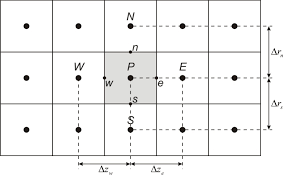
\includegraphics[width=60mm]{Imagens/malha.png}
	\caption{Exemplo de uma malha não adaptativa}
\end{figure}
%	\include{andre/}
%	\include{arturo/}
%   \include{denise/}
	\thispagestyle{empty} %Oculta o numero da primeira pagina do capitulo
\vspace{3ex}


\chapter{Estudo de viabilidade do método KPLS na predição de vida em fadiga.}
\label{finalsec}

\section{Introdução}
% O método KPLS (Kriging e médios quadrados parciais), quando usado na predição de séries temporais de tensão, pode resultar em boas aproximações a baixos custos computacionais.

Neste segmento procura-se estudar os impactos da utilização do método KPLS (\emph{Kriging model and partial least squares}) na predição de séries temporais de tensão para aplicação no estudo da vida em fadiga dos elementos estruturais. No caso deste estudo, a análise é feita a partir das tensões externas de Von Mises desenvolvidas a partir do software Anflex do CENPES/PETROBRAS. O caso analisado consiste em um longo \emph{riser} com flutuadores (Fig. \ref{figure.1}) que tornam flutuante parte da estrutura submersa (configuração \emph{lazy-wave}). 

\begin{figure}[!h]
    \centering
    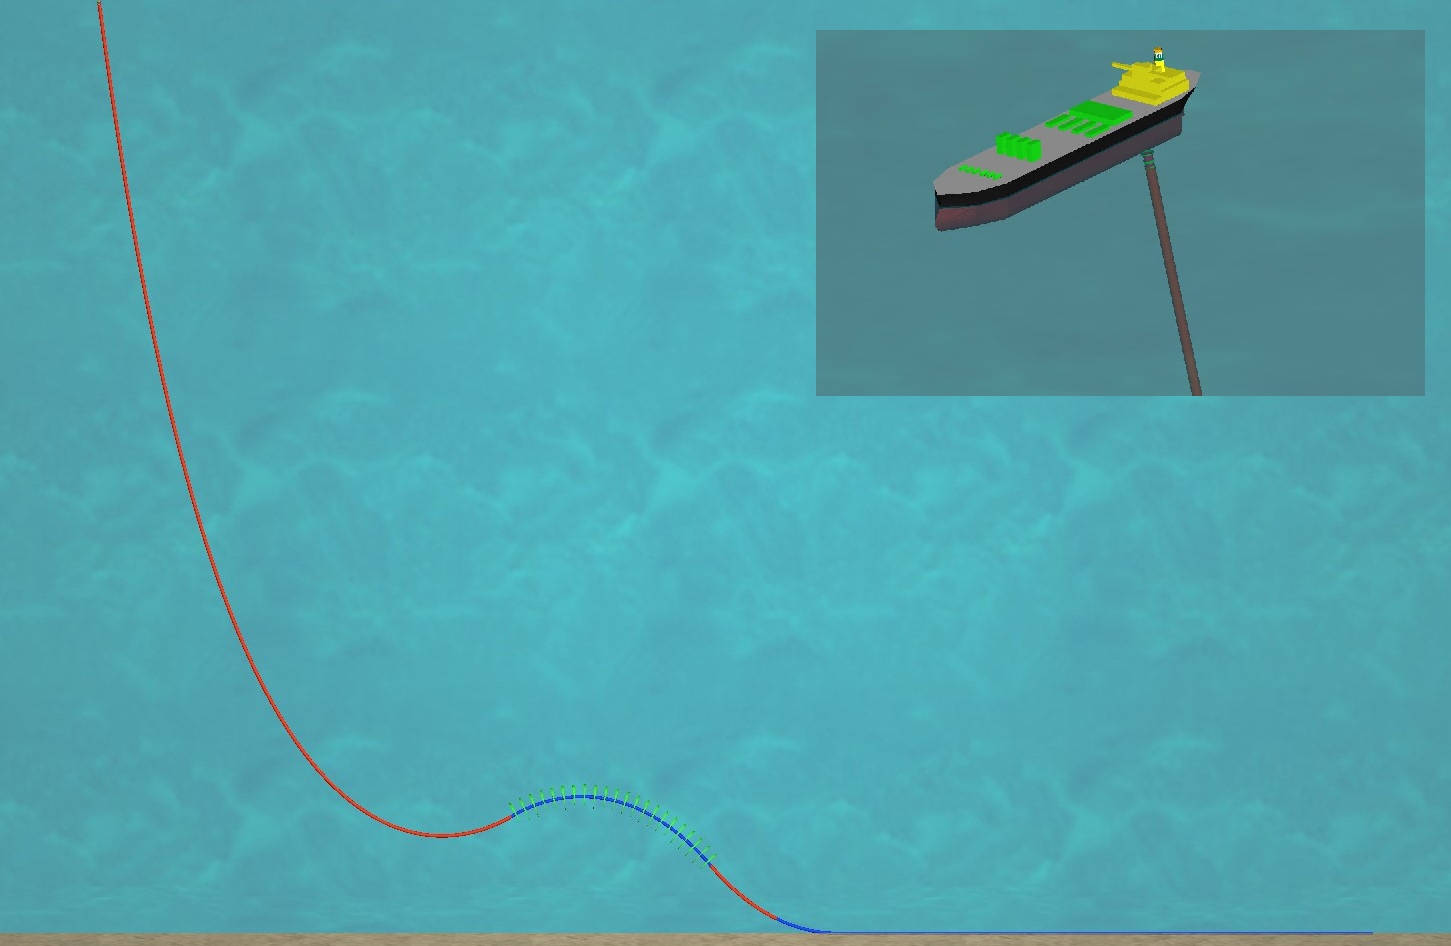
\includegraphics[width=0.5\linewidth , trim = {40mm 0mm 30mm 5mm} , clip]{felipe/fig_felipe/caso_estudado.jpg}
    \caption{Configuração \emph{lazy-wave}, onde o estudo foi desenvolvido.}
    \label{figure.1}
\end{figure}

O segmento flutuante (denominado região de SAG/HOG) tem o objetivo de atenuar os carregamentos advindos dos deslocamentos da estrutura flutuante ào segmento do riser em contato com o leito marinho. Seus efeitos podem ser observados no andamento deste estudo ao causar notável influencia na vida em fadiga dos elementos próximos. 

A biblioteca SMT foi utilizada para aplicação do método KPLS. Este pacote possui muitas ferramentas de metamodelo também aplicadas neste projeto \textbf{(BOUHLELet al., 2019)}.

Dessa forma, tem-se o intúito de se aplicar o método \emph{RainFlow} e o método de Goodman modificado para determinação da vida em fadiga a partir das séries de tensões externas de Von Mises advindas das simulações feitas no Anflex. O método KPLS é utilizado para predição parcial destas séries e então se calcula a vida em fadiga destas séries parcialmente ajustadas. Comparando-se os resultados observou-se boa conformidade, o que levanta boas oportunidades de otimização ao tornar facultativo o desenvolvimento de uma simulação completa para este tipo de análise. 

% Como mencionado, o pacote SMT foi utilizado para determinar os resultados deste relatório parcial. Os seguintes metamodelos est ̃ao disponíveis nesta biblioteca Python (BOUHLELet al., 2019)

% desenvolver um algorítmo com o qual se possa analisar a vida em fadiga a partir das séries temporais de tensão advindas do software Anflex. Além disso este programa deve ser capaz de fazer a predição de séries temporais de tensão a partir do médo KPLS. Dessa forma, com a rotina se comparará os valores de vida em fadiga a partir dos dados de tensão completamente simulados pelo Anflex e a partir dos dados parcialmente ajustados com o método KPLS.

\section{Metodologia}

\subsection{Método RainFlow}

\subsection{Método de Goodman modificado}

\subsection{Método KPLS de predição de séries temporais}

\subsection{Análise introdutória da vida em fadiga}




%	\include{helio/}
%	\include{marcelo/}
%	\include{tatiane/}

	\chapter{Conclusões e considerações finais}
		\label{finalsec}
		
		Este relatório técnico parcial teve como objetivo apresentar os desenvolvimentos realizados no período de junho de 2019 -- dezembro de 2019. Entre as principais contribuições compreendidas no mesmo, pode-se citar a revisão bibliográfica acerca de vários métodos de metamodelagem, a implementação computacional de algumas destas técnicas, bem como de procedimentos de amostragem, com posterior aplicação das mesmas em funções de teste bem difundidas na literatura, o êxito na realização de prolongamentos de séries temporais advindas de simulações realizadas com o \textit{software} Anflex e, por fim, a validação da ferramenta computacional MFSim através da comparação dos sinais de CD e CL obtidos com dados provenientes de experimentação material.
		
		\begin{equation}
			\frac{1}{2}
		\end{equation}







		
	\begin{singlespace}
		\phantomsection
		\addcontentsline{toc}{chapter}{Referências Bibliográficas}
		 %\bibliographystyle{acm}
		% \bibliographystyle{plain}
		\bibliography{metamodelo}
	\end{singlespace}
	%\include{apendices}

\end{document}   % Fim.